%%% DOCUMENT SETUP %%%
\documentclass[11pt,a4paper,onecolumn]{article}
\usepackage[greek,english]{babel}

%%% LAYOUT %%%
\usepackage{fullpage}
\usepackage[parfill]{parskip}
\usepackage{multicol}
\usepackage{footnote}

%%% GRAPHICS %%%
\usepackage{graphicx}
\usepackage{color}
\usepackage{graphics}
\usepackage{rotating}
\usepackage{subfig}
\usepackage{amsmath}
\usepackage{amssymb}
\usepackage{amscd}
\usepackage{xfrac}
\usepackage{float}
\usepackage{dsfont}

%%% FONT %%%
\usepackage{ifxetex}
\ifxetex
  \usepackage{fontspec}
    \setmainfont{Linux Libertine O}
  \usepackage{xunicode}
  \usepackage{microtype}
\else
  \usepackage[T1]{fontenc}
  \usepackage[latin1]{inputenc}
  \usepackage{times}
  \usepackage{microtype}
\fi

%%% Coding %%%
\usepackage{listings}
\usepackage{pseudocode}

%%% TITLE PAGE %%%
\author{Jeroen Hofman (2513225) \\
  [15pt] Vrije Universiteit (\textsc{VU})
}

\title{Data Mining Techniques \\
  Assignment 1
		}

\begin{document}
\maketitle
\captionsetup{width=0.8\textwidth}
\lstset{language=Python,breaklines=true,backgroundcolor=\color{white},frame=single}
\thispagestyle{empty}

\newpage

\section{Introduction}
In this small report we explore and classify some data generated in class. We look at different relations, which might or might not exist, and discuss briefly some features of the used software RapidMiner. I have chosen this software since I am unfamiliar with it. The structure of the report is somewhat vague compared to a regular report, because of the somewhat ill-defined task of exploration.

\section{Exploration}
In this section we have tried out several features of RapidMiner, starting by loading the data and examining it more closely. The meta data view reveals the following interesting features about participants of the survey:

\begin{itemize}
\item 
  There is a total number of 67 participants in the survey, of which 25 are studying BMI.
\item
  More than 50\% of participants have followed a course in machine learning, statistics and databases, the course on information retrieval is less popular.
\item
  'Your birthday' has been interpreted in 2 ways, either with birth year or without (though technically it is without, but it is hard to hear if someone is saying 'birthday' or 'birthdate')
\item
  The majority of participants did not stand up, although the missing values are large in number. This indicates most people were not very thrilled with the 9 o'clock lecture.
\item
  Both for the stress level and the money question one participant entered high numbers, hence producing basic statistics (range, average) which are not reliable.
\item
  The random number is surprisingly close to the expected average ((10 + 1) / 2 = 5.5), however, the value 13 was also reported.
\end{itemize}

Of course the metadata can only tell us so much, we have picked several topics to explore a bit more in detail. We would expect there to be a certain trend in the sleeping time, the stress level and the amount of drinks last night. Namely, we expect participants who entered a large amount of drinks to sleep later, but have diminished stress levels. Figure \ref{fig:sleeptime} below shows a scatter plot of the stress level versus the sleeping time, where the color of the dots indicates the amount of drinks.

\begin{figure}[h]
  \centering
  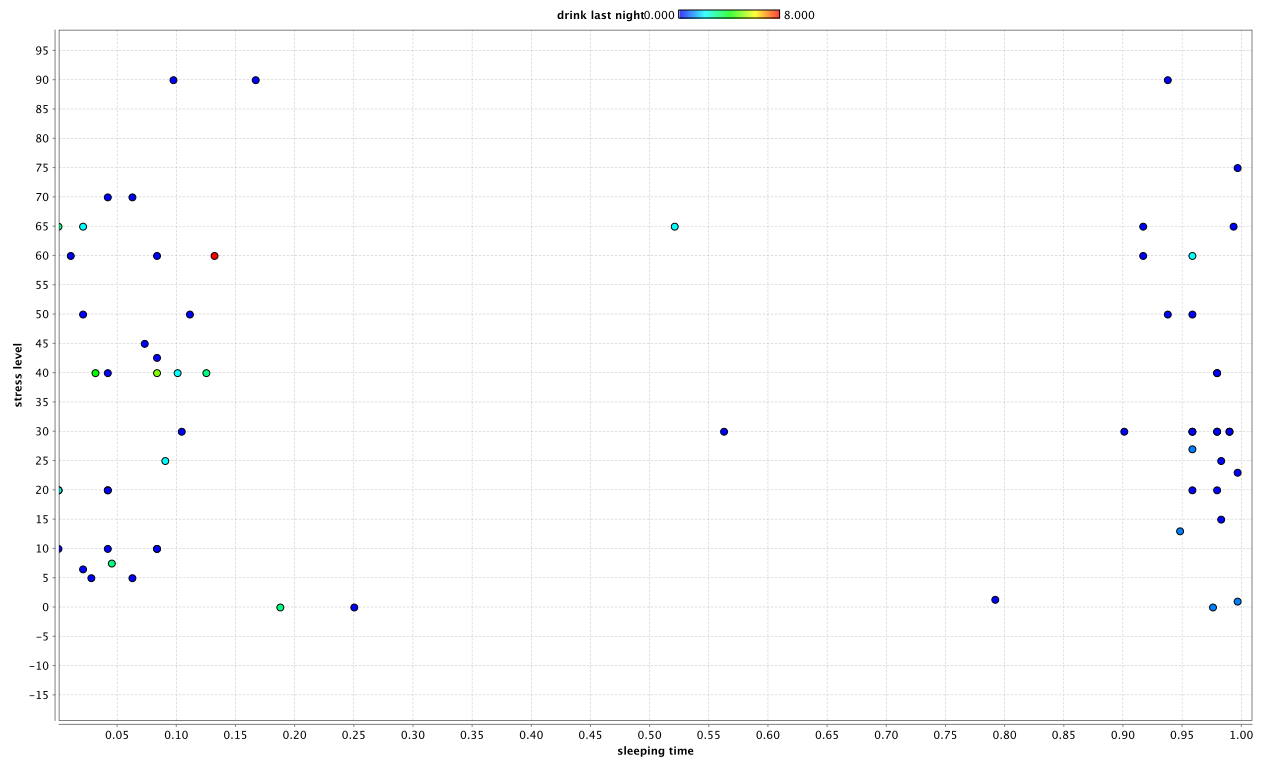
\includegraphics[width=0.9\textwidth]{sleeptime.png}
  \caption{The stress level versus sleeping time, the color of the dots gives the number of drinks.}
  \label{fig:sleeptime}
\end{figure}

From the figure there does not seems a relation between sleeping time and stress level, since the distribution is flat as a function of sleeping time. However, there seems to be a link to the number of drinks and the sleeping time. Note that there are roughly two groups, the left group corresponds to sleeping after midnight, the right group corresponds to sleeping before midnight. The left group has a higher average drinking than the right group, so there seems to be a relation between sleeping time and drinking. This is logical, since most people drink with others, so that is either hanging out or a party, in which case the time the event ends is often late (later then the normal sleeping time). We will investigate this in more detail in the next section.

Another interesting relation to explore is the question about the gorilla and the program the participants are in. Figure \ref{fig:gorilla} below shows a histogram where every pair of bins is a program, indicating how many of each program saw the gorilla and how many did not. I personally did not see any gorilla and since I was paying attention, most likely there was not a gorilla displayed. Interestingly though, not everyone is sharing that opinion and six people from AI did see a gorilla, which is rather remarkable. However the majority of people did not see a gorilla.

\begin{figure}[H]
  \centering
  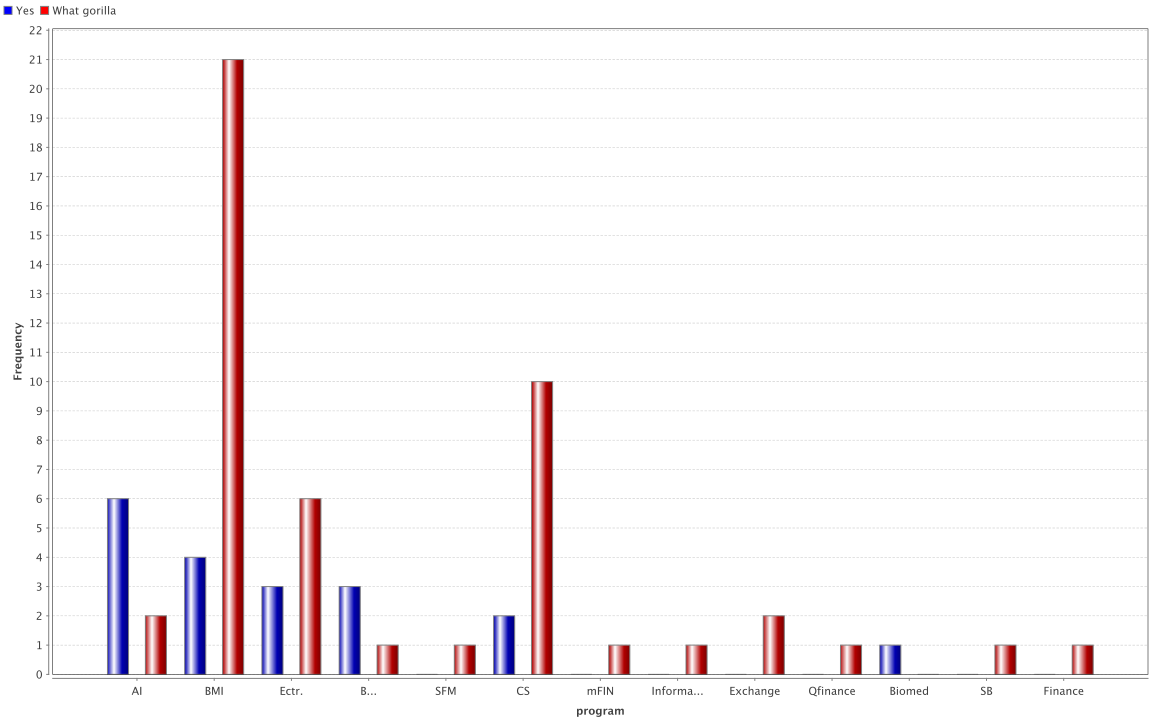
\includegraphics[width=0.9\textwidth]{gorilla.png}
  \caption{The amount of participants that observed a gorilla as a function of the program in which they are enrolled.}
  \label{fig:gorilla}
\end{figure}

Lastly for the exploration part we investigated whether the probability of taking a statistics course can be accurately predicted or not. A decision tree is shown below, see figure \ref{fig:stat}, deciding whether or not a participant attended a statistics course. Since most of the participants (61/67) took a statistics course, it is interesting whether there are certain features of the ones who did not take such a course, the results are given below.

\begin{figure}[h]
  \centering
  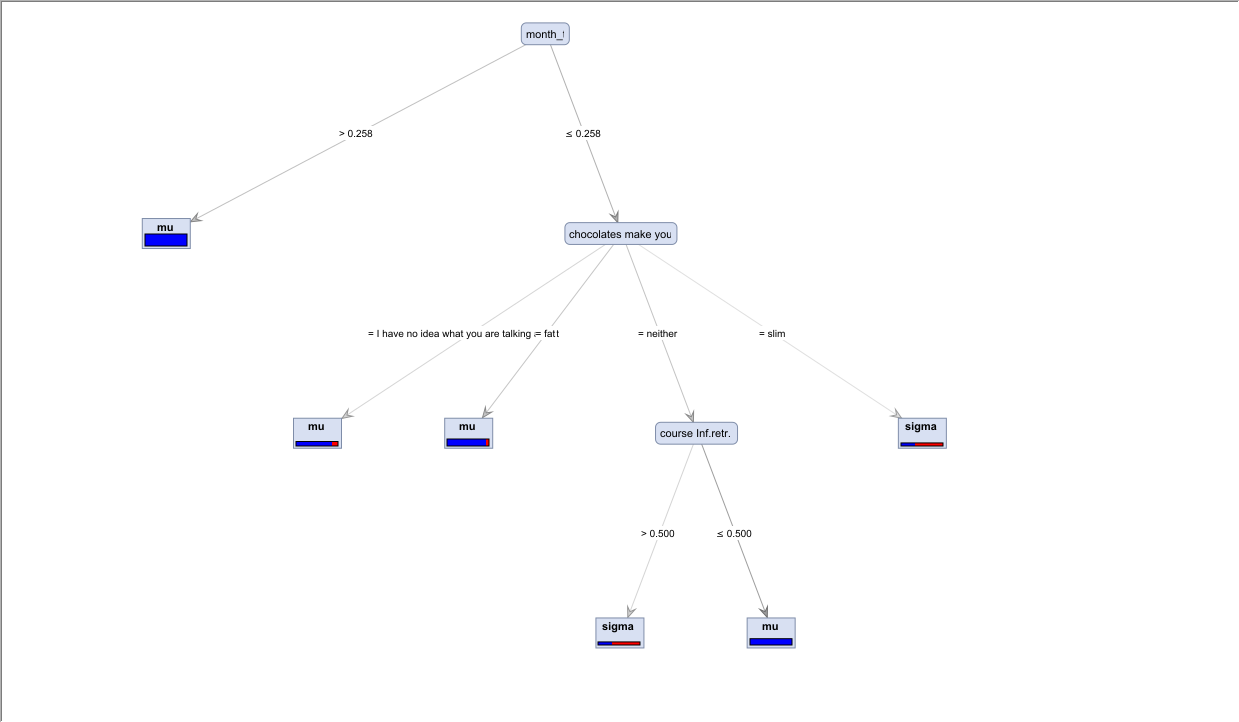
\includegraphics[width=0.9\textwidth]{statistics.png}
  \caption{Decision tree for the question: "Did you follow any course in statistics?"}
  \label{fig:stat}
\end{figure}

The tree shown in the figure is small, because only 6 participants have to be evaluated. Interestingly all 6 participants are born in a relativily 'late' month. The next branch in the tree relates to the chocolate question, if the answer is 'neither' a third branch is needed about the course in information retrieval. From this subset if the participant did not attent information retrieval, it did take a course in statistics (with an error of 0). This tree is of course not very useful because of the small number of people who is not attending this course, however most classes do not produce nice trees, since most non-numerical classes are heavily biased towards an attribute (or Rapid Mining refuses to make a decision tree).

\section{Classification/regression}
In the second part of the assignment we do a linear regression experiment, verifying it with cross-validation. Since a linear regression experiment only makes sense on data with some range of values (so no binomial type for instance), we choose the 'number of drinks last night' attribute together with the 'sleeping time' which we also briefly discussed in the previous section. The data for the sleeping time is slightly adjusted for values after midnight, all those values are incremented by one to reflect the fact that after midnight (>1) is later than before midnight (<1). We then proceed by building the following model (in RapidMiner):

\begin{itemize}
\item 
  Load the data set with the adjusted values for the 'sleeping time'.
\item
  Select the attributes 'sleeping time' and 'number of drinks last night'.
\item
  Replace any missing values in the data set by the average of the attribute in which the value is missing.
\item
  Set 'sleeping time' as the label, i.e. the input parameter $X$ for the linear regression $Y = A1 + A2 X$.
\item
  Perform linear regression with cross validation on the data set. The set is divided into 10 subsets after which one subset is picked, the training is performed on the other 90\% of the set and the validation is performed on that particular subset. This is then repeated for all subsets, so 10 times in total. The validation is performed by applying the model to the 'sleeping time', which gives an expected 'number of drinks last night'. This expected value is then compared to the observed value and the squared error is computed (the square of the difference between the two). This is done for all entries in the subset, then the average of the squared errors is computed and the square root is taken of this quantity. This is one of the most often used methods for calculating this error, also known as the root-mean-squared-error.
\end{itemize}

By executing this model we obtain the following relevant properties of the regression analysis:

\begin{itemize}
\item 
  The coefficient is 2.469 with a standard error of 1.533. This indicates that there is a positive correlation between the 'sleeping time' and 'number of drinks last night', i.e. the later participants went to bed, the more they had been drinking.
\item
  The p-value is 0.139, indicating that the probability of finding these values above considering the null-hypothesis to be true (i.e. coefficients 0, no correlation) is 14\%. Usually the allowed value for p is 0.05 or 0.01, so this value is high, indicating that the test does not give conclusive proof of the correlation that has been found in the point above, since when there is no correlation there is still a significant probability of finding these coefficients.
\item
  The intercept value is -1.842 with a standard error of 1.597, this is the constant value in the linear regression.
\item
  The performance vector (the root-mean-squared-error) that was calculated is 1.383 $\pm$ 0.660. This vector can be used to compare with other models, in general a smaller value for the performance vector indicates that the regression results give a better prediction of the data. The error in the vector comes from the calculation of performance vectors for every subset, because these vectors will not be the same.
\end{itemize}

The fact that this regression does not give conclusive results could also already have been predicted by just looking at the values and the error of the coefficients. A good rule of thumb is that values within two times the standard error with respect to coefficient are still likely, in this case this would also include zero, which is the null hypothesis. 

The data was obtained on a Tuesday morning, hence the question applied to a Monday evening, which is not a night many people drink, this is also reflected by the fact that a large portion of the people (48 out of 67) did not drink that night. The correlation might have been more clear on for example a Friday night, where people go out and drink and then stay up late, whereas some people might not go out, hence probably will not drink (or drink less) and go to bed earlier.

As comparison to this algorithm, we took a very similar algorithm, namely the polynomial regression. The model stays the same but instead of modelling $Y = A1 + A2 
X$, we now fit the data to a polynomial function. We fitted the data to a polynomial of degree 3, i.e. of the form $Y = A1 + A2 X + A3 X^2 + A4 X^3$ (with 5000 iterations). The values found are $A1 = 16.368, A2 = 0, A3 = -34.978$, and $A4 = 19.402$. With this model the performance vector has a value of 1.237 $\pm$ 0.715, which is slightly better than the linear regression but to the expense of a much longer computation time. Also the error is slightly larger in the case of polynomial regression.

\section{Conclusion}
In the first part we looked at general properties of the dataset, which did not reveal many interesting patterns. In the second part we investigated regression between the 'sleeping time' and 'number of drinks'. We found a positive correlation for linear regression, which is however not very reliable. We also performed a polynomial regression and found a slightly better fit, which was however still not very reliable.

\end{document}

